\section{Análise comparativa}\label{comparativa}
\esb{em todos exp, a necessidade de aplicação de filtro é separada, ex.: o learner precisa,
mas não obriga o classif a usar ou viceversa;
a mesma ideia foi estendida para a relação estrat-learner,
a estratégia precisa (maha), mas não obriga o learner a usar  ou viceversa}

Há aplicações cujas particularidades ou preferências do especialista determinam
previamente o algoritmo de aprendizado. \ano{exemplos?}
Nessas aplicações, o algoritmo do classificador coincide com o algoritmo do aprendiz.
Por outro lado, há aplicações em que a escolha do algoritmo é livre e, definido o
aprendiz (ou sua ausência), a escolha do classificador se dá idealmente a partir do
momento em que o conjunto de treinamento se torne suficientemente grande para
a realização de uma validação cruzada \ano{ref?}.
Para simular esses dois cenários de forma concisa,
a comparação de estratégias está dividida da seguinte maneira:
\begin{enumerate}
  \item \textbf{algoritmo pré-definido} -
  cada combinação base-algoritmo é um teste e cada estratégia é uma abordagem sob comparação;
  o desempenho é medido durante a evolução do aprendiz.
  \item \textbf{algoritmo definido após rotulação} -
  cada base é um teste e cada par estratégia-aprendiz é uma abordagem sob comparação;
  o desempenho é medido com o melhor classificador obtido após a rotulação.
\end{enumerate}

\subsection{Cenário com algoritmo pré-definido}\label{predefinido}
\ano{detalhes do exp aqui ou na metodologia ou nos dois?:
ALC kappa}

No cenário em que o algoritmo a ser adotado pelo aprendiz e pelo classificador é
pré-definido, supõe-se que a aplicação impõe
o algoritmo a ser usado devido à natureza do problema ou devido a restrições do sistema; ou,
o especialista recorre à experiência pessoal ou faz uma escolha arbitrária.
Assim, todas as combinações base-algoritmo foram consideradas possíveis numa aplicação real
e puderam ser adotadas como testes no experimento.

% http://research.cs.wisc.edu/techreports/2009/TR1648.pdf
Estratégias são normalmente avaliadas por meio de curvas de aprendizado,
que são os gráficos da medida de interesse em função da quantidade de consultas
\citep{settles2010active}.
% Figure 3 presents learning curves for the first 100 instances labeled using
% uncertainty sampling and random sampling.
% The reported results are for a logistic regression model averaged over ten folds
% using cross-validation.
O comportamento típico da curva de aprendizado ativo seguido pelas diferentes estratégias
é ilustrado na Figura \ref{curvas}
Apesar da pouca discernibilidade das curvas, a exibição delas permite notar
que elas têm a mesma forma logarítmica, com o valor kappa divergindo na medida em que novos
exemplos são consultados.
\input plot
Se todas as bases tivessem a mesma quantidade de exemplos
e o aprendizado prosseguisse, as curvas se encontrariam novamente,
pois tendem ao desempenho passivo.

É possível observar que a curva de SVMbal se destaca negativamente,
mas comparações de curvas neste gráfico são imprecisas devido aos diferentes
pesos que as bases podem ter:
bases mais difíceis, por exemplo, tendem a ter um valor mais baixo para kappa e acabam
sub-representadas.
Uma forma de neutralização desse tipo de desigualdade entre as bases é a adoção
de ranqueamento das médias\footnote{Além das médias,
um gráfico das medianas também foi elaborado e teve um comportamento praticamente igual.
% com leves perturbações irrelevantes
Por motivos de espaço ele foi omitido.}, conforme mostrado na Figura \ref{curvasrank},
que confirma o mau desempenho de SVMbal e QBCRFw - as duas estratégias de aprendiz fixo.
\input rankplot
Os aprendizes fixos (SVM e RFw) podem gerar consultas desfavoráveis aos outros algoritmos
empregados como classificador (5NN, C4.5w, CIELM e NB).
De forma mais ampla, pode-se esperar que estratégias gnósticas não tenham um desempenho
constante ao longo de todos os seis aprendizes em cada base.
Essa hipótese seria mais provável se as estratégias agnósticas (Rnd, Clu e ATUmah) tivessem obtido
resultados acima da média, porém Rnd e Clu que permaneceram
abaixo da colocação média ($5.5$) por praticamente todo o intervalo de consultas.
ATUmah se manteve próxima da média, porém com mais vantagem na primeira metade do orçamento.
Assim, é mais provável que a própria natureza das estratégias seja inferior para o dado conjunto de bases.
\ano{muito especulativo}

% DWeuc é a estratégia Mar ponderada pela densidade, logo, dada a superioridade de Mar,
% a ponderação por densidade pode ser considerada bastante prejudicial quando não leva em
% conta os exemplos rotulados.
% Por outro lado, as extensões de DW (TU, ATU e GATU) superam as demais, pois ponderam inversamente pela
% densidade de exemplos rotulados evitando, assim, as regiões densamente rotuladas.
SGmulti, por sua vez, se manteve estável, pouco acima da colocação média.
Um evento importante entre as melhores curvas é a inversão entre a estratégia agnóstica
ATUmah e Mar após aproximadamente $50$ exemplos.
Essa inversão coincide com a intuição de que consultas exploratórias sejam vantajosas no início do
aprendizado, enquanto que consultas prospectivas passem a ser proveitosas mais tardiamente.
Assim, estratégias como HTUmah e TUmah, capazes de combinar agnosticidade e gnosticidade,
podem ter um bom desempenho tanto no início quanto no restante da curva de aprendizado
conforme evidenciado por suas curvas.
A curva ascendente de Mar, quando vista isoladamente, também é um indicativo de que a prospecção pura
é prejudicial no início e vantajosa com o avanço do aprendizado.
Por fim, EERent mostrou-se como uma das melhores opções pela estabilidade e colocação de sua curva.

Para confirmar as conclusões com segurança estatística, os níveis de confiança
($p \in \{0,01; 0,05; 0,10\}$) na Tabela \ref{stratsALCKappaFriedAllReduxall} indicam
quando uma estratégia na linha é melhor que a outra na coluna.
O critério de vitória é baseado na comparação dos valores da kappa médio para todas as bases.
A medida foi calculada com $200$ exemplos nas bases de tamanho suficiente
e $|\mathcal{U}|$ nas demais.
% \input stratsmahALCKappaFriedAllReduxall
\begin{table}[h]
\caption{Um contra um para as estratégias (564 testes).
Medida: kappa médio. \textit{Legenda na Tabela \ref{tab:friedClassif}.}}

\begin{center}
\scalebox{0.82}{
\begin{tabular}{lcc|cc|cc|cc|cc}
                   & 1 & 2 & 3 & 4 & 5 & 6 & 7 & 8 & 9 & 10\\
1 - Rnd         & - &   &   &   &   &   &   &   &   &   \\
2 - Clu         & + & - &   &   &   & * &   &   &   & * \\ \hline
3 - \textbf{ATUmah}     & * &   & - &   &   & * &   &   &   & * \\
4 - \textbf{HTUmah}     & * & * & * & - & * & * &   &   &   & * \\ \hline
5 - \textbf{SGmulti}    & * &   &   &   & - & * &   &   &   & * \\
6 - QBCRFw      &   &   &   &   &   & - &   &   &   &   \\ \hline
7 - Mar         & * & * &   &   &   & * & - &   &   & * \\
8 - TUmah       & * & * & + &   & + & * &   & - &   & * \\ \hline
9 - EERent      & * & * & * &   & * & * &   &   & - & * \\
10 - SVMbal     &   &   &   &   &   &   &   &   &   & - \\ \hline
\end{tabular}
}
\quad
\scalebox{0.82}{
\begin{tabular}{lccc}
algoritmo & \makecell{primeiros\\lugares} & \makecell{derrotas\\para Rnd}  & \makecell{últimos\\lugares} \\
\hline
EERent     & \bom{280} & \bom{168} & 121 \\
\textbf{HTUmah}     & \bomd{251} & \bomd{179} & \bom{88} \\
Mar        & 235 & 187 & 161 \\
TUmah      & 233 & 200 & \bomd{119} \\
\textbf{ATUmah}     & 176 & 207 & 139 \\
\textbf{SGmulti}    & 152 & 216 & 134 \\
SVMbal     & 123 & \ruim{334} & \ruim{304} \\
QBCRFw     & 106 & 311 & 266 \\
Clu        & 103 & 227 & 164 \\
Rnd        & \ruim{71} & - & 225 \\
\end{tabular}
}
\label{stratsALCKappaFriedAllReduxall}
\end{center}
\end{table}

Como um indicativo da viabilidade do aprendizado ativo em geral, Rnd perde de todas exceto QBCRFw
e SVMbal.
Clu superou a amostragem aleatória, respeitando a garantia teórica de que não é inferior a ela.
Dentre as melhores estratégias,
a proposta HTUmah obteve vitórias maior significância estatística que sua principal contendente TUmah
e se equiparou a EERent.
Dentre as agnósticas selecionadas ATUmah é a preferível, também por superar suas contendentes
significativamente.
SGmulti obteve um desempenho próximo ao de ATUmah.

% Se forem consideradas apenas as primeiras 100 consultas -
% %150 conf/emnlp/SettlesC08
% valor arbitrário frequentemente adotado em outros trabalhos
% \citep{journals/pieee/CrawfordTY13,chermanaprendizado,conf/nips/SettlesCR07,conf/icml/RoyM01} -
% A comparação passa a ser como na Tabela \ref{stratsALCKappaFriedAllReduxHalf}.
% \input stratsmanALCKappaFriedAllReduxall
% \input stratseucALCKappaFriedAllReduxall
% conforme Tabela \ref{stratsALCKappaFriedAllReduxHalf}.
% $50$ exemplos: quantidade máxima antes que o tamanho das bases permita ALCs de tamanhos diferentes
% - conforme Tabela \ref{stratsALCKappaFriedAllRedux50}.
Em aplicações reais, entretanto, a estabilidade do algoritmo pode ser mais importante
do que o desempenho preditivo médio, pois uma grande variabilidade pode colocar o
orçamento sob o risco de ser gasto sem que seja atingido um desempenho adequado e pode levar a custos
excedentes de rotulação imprevisíveis.
Assim, a estabilidade da estratégia tem fundamental importância para a análise do risco financeiro
da aplicação. É importante enfatizar que o processo de rotulação é irreversível,
impossibilitando a experimentação de mais de uma estratégia.

De forma análoga às curvas apresentadas para o valor médio de kappa e o ranqueamento
correspondente, dois conjuntos de curvas baseadas no desvio padrão do valor de kappa foram
construídos visando ilustrar o comportamento da variância preditiva a cada instante ao longo
de sucessivos valores de orçamento.
É possível observar, na Figura \ref{curvasrankdesvio}, que as estratégias ATUmah, HTUmah,
TUmah e EERent detêm as melhores colocações no ranqueamento médio dos menores valores de desvio
padrão durante a maior parte do processo de rotulação.
\input rankplotRisco
\input plotRisco
O mesmo ocorre com os ranqueamentos apresentados na Figura \ref{curvasdesvio}.
Nesse gráfico, a distância entre a melhor e a pior curva se mantém em torno de $0,01$,
indicando que, embora algumas sejam mais estáveis, a faixa ocupada pelas curvas é estreita.
porém com EERent alternando com TUmah.
A curva de SGmulti ficou em torno do ranqueamento médio ($5,5$).

Uma propriedade das curvas é a tendência de estabilização durante o treinamento,
indicando que em baixos orçamentos a escolha de estratégias mais estáveis é prioritária.
A significância estatística das diferenças pode ser verificada na Tabela
\ref{stratsALCKappaFriedAllRiscoReduxall}.
\begin{table}[h]
\caption{Um contra um para as estratégias. Medida: desvio padrão do kappa médio. \textit{Legenda na Tabela \ref{tab:friedClassif}.}}
\begin{center}
\begin{tabular}{lcc|cc|cc|cc|cc}
                                  & 1 & 2 & 3 & 4 & 5 & 6 & 7 & 8 & 9 & 10\\
1 - Rnd                        & - &   &    &   &    &   &    &    &   &   \\
2 - Clu                         &   & - &    &   &    &   &    &    &   &   \\ \hline
3 - \textbf{ATUmah}     & *& * & -  &   & * &   & * &    & * & * \\
4 - \textbf{HTUmah}     & * & * &   & - & * &   & * &  +& * & * \\ \hline
5 - \textbf{SGmulti}       &   &   &    &   & - &   &    &   &   &   \\
6 - QBCRFw                 & * & * &    &   & * & - & * &   & * & * \\ \hline
7 - Mar                        &   &   &    &   &    &   &  - &    &   &   \\
8 - TUmah                   & * & * &    &   & * &   & * &  - & *& * \\ \hline
9 - EERent                   &   & * &    &   &    &   &    &    & - &   \\
10 - SVMbal                 &   &   &    &   &    &   &    &    &   & - \\ \hline\end{tabular}
% calculado pelo R
\label{stratsALCKappaFriedAllRiscoReduxall}
\end{center}
\end{table}

Finalmente, pode-se concluir que a versão híbrida proposta (HTUmah) é superior a TUmah
para o conjunto de bases e algoritmos utilizados.
ATUmah é viável enquanto alternativa agnóstica.
SGmulti obteve um desempenho mediano,
logo ela pode ser uma candidata a viés de amostragem alternativo num sistema de recomendação.
Com relação à minimização de risco financeiro, 
novamente as estratégias propostas também se mostraram viáveis,
com HTUmah sendo a mais estável - vencendo TUmah com significância estatística.

A principal dificuldade do cenário explorado nesta seção é, possivelmente, a existência de algumas
combinações menos favoráveis entre as bases e os algoritmos selecionados.
Algumas delas são perceptíveis na Figura \ref{treebadleas}.
A árvore indica a contagem de derrotas de cada algoritmo de acordo com a medida kappa.
Pequenas reservas de exemplos ($\#exemplos \leq 142,4$),
por exemplo, desfavorecem CIELM mais fortemente.
% \afterpage{\clearpage\begin{landscape}
\begin{figure}
\tikzset{
every node/.style={font=\scriptsize,black, thin},
decision/.style={shape=rectangle, minimum height=1cm, text width=1.7cm,
text centered, rounded corners=1ex, draw},
outcome/.style={ shape=rectangle, fill=red!15, draw, text width=2cm, text justified},
decision tree/.style={sibling distance=3cm, level distance=2cm},
cond/.style={blue, yshift=-2mm, shape=rectangle, text centered},
}
\begin{center}
\caption{Possíveis nichos de inadequação base-algoritmo.
\textit{Mínimo de dez exemplos por folha.}}
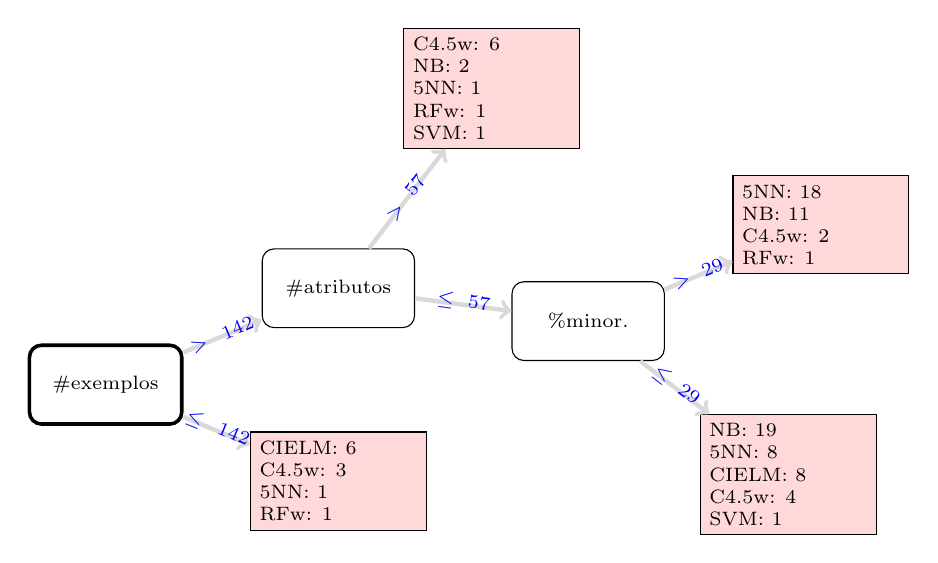
\begin{tikzpicture} [edge from parent/.style={->,above,draw,sloped,midway,gray!30,ultra thick},
text width=2.7cm, align=flush center, grow cyclic,
level 1/.style={level distance=3.2cm,sibling angle=45},
level 2/.style={text width=2cm, font=\footnotesize, level distance=3.2cm,sibling angle=60},
level 3/.style={text width=2cm, font=\footnotesize, level distance=3.2cm,sibling angle=60},
level 4/.style={text width=2cm, font=\footnotesize, level distance=3.2cm,sibling angle=60},
level 5/.style={text width=2cm, font=\footnotesize, level distance=3.2cm,sibling angle=60},
]
\node[line width=0.3ex, decision] {\#exemplos}
child {node [outcome] {CIELM: 6\\
C4.5w: 3\\
5NN: 1\\
RFw: 1} edge from parent node [cond] {$\leq142$}}
child {node [decision] {\#atributos}
child {node [decision] {\%minor.}
child {node [outcome] {NB: 19\\
5NN: 8\\
CIELM: 8\\
C4.5w: 4\\
SVM: 1} edge from parent node [cond] {$\leq29$}}
child {node [outcome] {5NN: 18\\
NB: 11\\
C4.5w: 2\\
RFw: 1} edge from parent node [cond] {$>29$}}edge from parent node [cond] {$\leq57$}}
child {node [outcome] {C4.5w: 6\\
NB: 2\\
5NN: 1\\
RFw: 1\\
SVM: 1} edge from parent node [cond] {$>57$}}edge from parent node [cond] {$>142$}};
\label{treebadleas}
\end{tikzpicture}
\end{center}
\end{figure}
% \end{landscape}\clearpage}

\subsection{Síntese das comparações}\label{sintese}
\ano{rever}
\tar{fazer uma sintese pra cada uma das duas comparações ou fazer uma sintese só no fim de tudo?}
Estratégias agnósticas têm a vantagem de dispensar o aprendiz.
Assim, elas evitam o risco de uma escolha inadequada de algoritmo de aprendizado
para um dado problema.
Consequentemente, ATUmah seria a preferível no caso de algoritmos variados.
Entretanto, os resultados dos quatro experimentos apontam para diferentes melhores
estratégias.
Apesar de ATUmah não ter sido pior que a amostragem aleatória em nenhum deles,
ela perde de Mar, TUmah e EERent em alguns casos.
Logo, se for desejado o melhor desempenho para um dado algoritmo,
então é preciso recorrer a algum procedimento que minimize a chance de
uma escolha inadequada de estratégia.
Além do algoritmo, o orçamento disponível e as características de cada base também
podem favorecer ou prejudicar certas estratégias.

Nesta seção, as estratégias são comparadas com o objetivo de identificar nichos
em que umas possam se sobressair em relação às outras.
Cada nicho corresponde a um algoritmo e um conjunto de bases de dados similares entre si.

Nas árvores exibidas nas figuras \ref{treeBest} e \ref{tree},
é possível observar o papel central do algoritmo de aprendizado sobre
a estratégia de aprendizado ativo, pois é a primeira regra em ambas as árvores.
Elas simulam dois cenários com relação à escolha do algoritmo: quando o mais adequado é conhecido
(\ref{treeBest}) e quando ele é arbitrário (\ref{tree}).
O primeiro caso resulta em $95$ metaexemplos devido a um empate,
e o segundo caso também resulta em torno de $95$ metaexemplos, porém para cada algoritmo,
totalizando $595$.
% Apesar de ilustrativa, a árvore pode não ser segura do ponto de vista de tomada de
% decisão devido ao baixo grau de pureza das folhas.
% \input arvorebest
% \input arvore
% \input arvorebestperd
% \input arvoreperd

% \ref{tree}
A amostragem aleatória aparece apenas na folha que representa o uso do 5NN nas quatro bases que têm
uma proporção de atributos nominais não muito alta (igual ou abaixo de $77$),
poucos atributos em geral (igual ou abaixo de $6$) e não muitos exemplos (igual ou abaixo de $1078$).
Assim, pode-se concluir que não optar pelo aprendizado ativo raramente é a melhor estratégia.
Num nicho similar, porém com muitos exemplos (acima de $1078$), HTUmah é a mais indicada.
ATUmah

% \ref{treeBest}
O algoritmo NB produz estimativas de distribuição de probabilidade excessivamente confiantes
que podem ser amenizadas por um \ing{comitê por amostragem}{bagging} \citep{conf/icml/RoyM01}.
Estratégias que dependem dessas estimativas podem ser prejudicadas.
ATUmah por ser agnóstica é independente dessas estimativas e aparece como nó
folha para esse algoritmo de aprendizado.
EERent também aparece e é gnóstico,
mas seu uso da soma das entropias das estimativas de
probabilidade de todos os exemplos da reserva ameniza o efeito do excesso de confiança.

% Algumas ramificações aceitam explicações plausíveis:
% \begin{itemize}
%  \item
% 
% % \esb{When Does Active Learning Work?
% % confirma que atributos não-discretizados favorecem AL,
% % isso justifica z-score para qq classificador ?
% % (ao menos RF, SVM, log reg. e QDA usados no artigo).
% % usa apenas QBC, entropia e random.
% % }
% \end{itemize}

\section{algoritmo definido após rotulação}\label{ind}
Numa aplicação real, a disponibilidade de rótulos permite uma escolha mais adequada
do algoritmo de aprendizado.
\ano{relembrar que U=100, o valor comum na literatura e para não ficar com menos de 75 bases}
Na Figura \ref{treegoodstrats}, embora a árvore de nichos de inadequação contenha uma
previsível presença expressiva das piores estratégias em todos os nós, como as variantes DW*,
algumas estratégias bem sucedidas no primeiro experimento aparecem com a maior frequência
de derrotas em alguns nós, como é o caso de EERent no caminho
(fronteira=flexível) $\rightarrow$ (algoritmo=CIELM) $\rightarrow$ ($\#atributos \leq 18$)
com 24 derrotas.
Assim, mesmo estratégias com um bom desempenho geral podem ser contraindicadas em
bases ou aprendizes com determinadas características - dificultando a definição prévia
do par estratégia-algoritmo mais adequado.
% \afterpage{\clearpage\begin{landscape}
\begin{figure}
\tikzset{
every node/.style={font=\scriptsize,black, thin},
decision/.style={shape=rectangle, minimum height=1cm, text width=1.7cm,
text centered, rounded corners=1ex, draw},
outcome/.style={ shape=rectangle, fill=red!15, draw, text width=2cm, text justified},
decision tree/.style={sibling distance=3cm, level distance=2cm},
cond/.style={blue, yshift=-2mm, shape=rectangle, text centered},
}
\begin{center}
\caption{Possíveis nichos de inadequação base-estratégia-algoritmo.
\textit{Mínimo de dez exemplos por folha.}}
\begin{tikzpicture} [edge from parent/.style={->,above,draw,sloped,midway,gray!30,ultra thick},
text width=2.7cm, align=flush center, grow cyclic,
level 1/.style={level distance=3.2cm,sibling angle=180},
level 2/.style={text width=2cm, font=\footnotesize, level distance=3.2cm,sibling angle=60},
level 3/.style={text width=2cm, font=\footnotesize, level distance=3.2cm,sibling angle=60},
level 4/.style={text width=2cm, font=\footnotesize, level distance=3.2cm,sibling angle=60},
level 5/.style={text width=2cm, font=\footnotesize, level distance=3.2cm,sibling angle=60},
]
\documentclass[tikz]{standalone}
\usepackage{lmodern,mathptmx,amsmath}
\usepackage{pbox}
\usepackage{marvosym}
\usepackage{bm}
\usepackage{wasysym}
\usepackage{makecell}
\usepackage{graphicx}
\usepackage{icomma}
\usepackage{afterpage}
\usepackage{pdflscape}
\usepackage{rotating}
\usepackage{pgfplots}
% \usepackage[T1]{fontenc}
% \usepackage[utf8]{inputenc}
\usepackage{pgfplots}
\usepackage{amsopn}
\usepackage{amsfonts}
\usepackage{amsthm, amsfonts, amssymb}
\usepackage{fontspec}
\pgfplotsset{compat=1.10}
\usetikzlibrary{trees}
\usetikzlibrary{patterns}
\usepgfplotslibrary{fillbetween}
\usetikzlibrary{fadings}
\tikzfading[name=myfading, top color=transparent!0, bottom color=transparent!80]
\defaultfontfeatures{Mapping=tex-text}
\setmainfont[Mapping=tex-text]{Latin Modern Roman}
\DeclareMathAlphabet{\mathcal}{OMS}{cmsy}{m}{n}
\DeclareMathOperator*{\unidist}{U}
\DeclareMathOperator*{\cov}{cov}
\DeclareMathOperator*{\argmax}{arg\,max}
\DeclareMathOperator*{\argmin}{arg\,min}
\DeclareMathOperator*{\sk}{sk}
\DeclareMathOperator*{\ku}{ku}
\DeclareMathOperator*{\qnc}{\#nc}
\DeclareMathOperator*{\qnom}{\#no}
\DeclareMathOperator*{\qnum}{\#nu}
\DeclareMathOperator*{\qatt}{\#at}
\DeclareMathOperator*{\qexe}{\#ex}
\DeclareMathOperator*{\qexeatt}{\#ea}
\DeclareMathOperator*{\lgqexe}{lgex}
\DeclareMathOperator*{\lgqexeatt}{lgea}
\DeclareMathOperator*{\nom}{isnom}
\DeclareMathOperator*{\pno}{\%no}
\DeclareMathOperator*{\en}{en}
\DeclareMathOperator*{\corr}{cr}
\DeclareMathOperator*{\cn}{cn}
\DeclareMathOperator*{\cnk}{cnk}
\DeclareMathOperator*{\si}{si}
\DeclareMathOperator*{\sik}{sik}
\DeclareMathOperator*{\du}{du}
\DeclareMathOperator*{\duk}{duk}
\DeclareMathOperator*{\dime}{dim}
\DeclareMathOperator*{\info}{Inf_\theta}
\DeclareMathOperator*{\stratID}{ID_\theta}
\DeclareMathOperator*{\stratIDTU}{ID_{TU_\theta}}
\DeclareMathOperator*{\JS}{JS}
\DeclareMathOperator*{\at}{\bm{a}}
\DeclareMathOperator*{\simi}{sim}
\DeclareMathOperator*{\limiar}{limite}
\DeclareMathOperator*{\limiaring}{max}
\pgfplotsset{marst/.style={solid, violet, mark=*, mark options={solid, scale=1.4}, mark repeat=60}}
\pgfplotsset{sgst/.style={solid, thick, orange, mark=x, mark options={solid, scale=2}, mark repeat=60}}
\pgfplotsset{eerst/.style={solid, red, mark=square*, mark options={solid, scale=1.4}, mark repeat=60}}
\pgfplotsset{hsst/.style={dashed, black, mark=triangle*, mark options={solid, scale=1.4}, mark repeat=60}}
\pgfplotsset{tust/.style={solid, gray, mark=square, mark options={solid, scale=1.4}, mark repeat=60]}}
\pgfplotsset{rndst/.style={loosely dashed, olive, mark=triangle, mark options={solid, scale=1.4}, mark repeat=60}}
\pgfplotsset{atust/.style={dotted, mark=star, ultra thick, blue,  mark repeat=50, mark options={solid, scale=1.9}, mark repeat=60}}
\pgfplotsset{htust/.style={solid, thick, green!50!black, mark=10-pointed star, mark options={solid, scale=1.9}, mark repeat=60}}
\pgfplotsset{dwst/.style={solid, thick, gray, mark=diamond, mark options={solid, scale=1.4}, mark repeat=60}}
\pgfplotsset{eer2st/.style={solid, brown, mark=pentagon, mark options={solid, thick, scale=1.4}, mark repeat=60}}
\pgfplotsset{htu2st/.style={dotted, blue, mark=triangle, mark options={solid, scale=1.5}, mark repeat=60}}
\pgfplotsset{defst/.style={loosely dashed, thick, blue, no marks}}
\begin{document}
\tikzset{every node/.style={font=\scriptsize,black, thin}, decision/.style={shape=rectangle, minimum height=1cm, text width=1.7cm, text centered, rounded corners=1ex, draw},
outcome/.style={ shape=rectangle, fill=red!15, draw, text width=2.8cm, text justified},
decision tree/.style={sibling distance=3cm, level distance=2cm},
cond/.style={blue, yshift=-2mm, shape=rectangle, text centered}}
\begin{tikzpicture} [edge from parent/.style={->,above,draw,sloped,midway,gray!30,ultra thick},
text width=2.7cm, align=flush center, grow cyclic,
level 1/.style={level distance=3.9cm,sibling angle=90},
level 2/.style={text width=2cm, font=\footnotesize, level distance=3.6cm,sibling angle=90},
level 3/.style={text width=2cm, font=\footnotesize, level distance=3.6cm,sibling angle=60},
level 4/.style={text width=2cm, font=\footnotesize, level distance=3.2cm,sibling angle=60},
level 5/.style={text width=2cm, font=\footnotesize, level distance=3.2cm,sibling angle=60},
]
\node[line width=0.3ex, decision] {algoritmo}
child {node [outcome] {
EERacc: 141\\
DWeuc: 111\\
Mar: 110\\
DWman: 106\\
TUeuc: 75\\
HS: 71\\
TUman: 70\\
EERent: 54\\
% \textbf{HTUman}: 26\\
% \textbf{ATUeuc}: 25\\
% \textbf{ATUman}: 21\\
% \textbf{SGmulti}: 0\\
demais ($\leq 26$): 106} edge from parent node [cond] {5NNw}}
child {node [decision] {\%nominais}
child {node [outcome] {
DWman: 90\\
DWeuc: 88\\
EERacc: 69\\
Mar: 65\\
\textbf{HTUman}: 60\\
TUeuc: 60\\
\textbf{HTUeuc}: 53\\
TUman: 52\\
\textbf{ATUeuc}: 50\\
\textbf{ATUman}: 48\\
% \textbf{SGmulti}: 44\\
% EERent: 20\\
demais ($\leq 44$): 110} edge from parent node [cond] {$\leq0,6$}}
child {node [outcome] {
EERacc: 28\\
EERent: 20\\
HS: 20\\
Mar: 18\\
DWeuc: 16\\
DWman: 15\\
\textit{SGmulti}: 11\\
TUeuc: 10\\
\textbf{HTUeuc}: 6\\
\textbf{ATUman}: 6\\
\textbf{HTUman}: 6\\
TUman: 6\\
% TUman: 6\\
% \textbf{ATUeuc}: 5\\
demais ($\leq 6$): 5} edge from parent node [cond] {$>0,6$}}edge from parent node [cond] {NB}}
child {node [outcome] {
DWman: 146\\
DWeuc: 141\\
Mar: 78\\
EERacc: 65\\
EERent: 61\\
HS: 59\\
\textit{SGmulti}: 55\\
TUeuc: 50\\
TUman: 41\\
\textbf{ATUman}: 38\\
% \textbf{ATUeuc}: 36\\
% \textbf{HTUman}: 32\\
demais ($\leq 36$): 105} edge from parent node [cond] {C4.5w}}
child {node [decision] {\%minor.}
child {node [outcome] {
DWeuc: 31\\
DWman: 29\\
\textbf{HTUman}: 27\\
\textbf{ATUeuc}: 27\\
\textbf{ATUman}: 26\\
TUeuc: 25\\
TUman: 24\\
\textbf{HTUeuc}: 22\\
\textit{SGmulti}: 19\\
% EERacc: 8\\
% HS: 6\\
% EERent: 4\\
demais ($\leq 8$): 36} edge from parent node [cond] {$\leq7,6$}}
child {node [outcome] {
Mar: 102\\
DWman: 95\\
DWeuc: 91\\
TUeuc: 88\\
TUman: 84\\
\textbf{ATUman}: 78\\
\textbf{HTUman}: 74\\
\textbf{ATUeuc}: 68\\
\textbf{HTUeuc}: 66\\
EERacc: 58\\
% \textbf{SGmulti}: 47\\
% EERent: 41\\
demais ($\leq 47$): 141} edge from parent node [cond] {$>7,6$}}edge from parent node [cond] {SVM}}
;
\end{tikzpicture}
\end{document}
\label{treegoodstrats}
\end{tikzpicture}
\end{center}
\end{figure}
% % \end{landscape}\clearpage}
Mesmo que o usuário disponha de informações auxiliares sobre o domínio da aplicação,
elas podem não se aplicar ao seu conjunto específico de exemplos cujo tamanho foi restringido
pelo orçamento, pois algoritmos com boa performance em treinamento com poucos
dados podem ter baixa performance com muitos dados
\citep{journals/sigkdd/AttenbergP10,journals/jmlr/PerlichPS03}.
Assim, estratégias agnósticas e aquelas cujo aprendiz possa ser desvinculado da escolha do
algoritmo de aprendizado definitivo da aplicação se mostram desejáveis.

As estratégias agnósticas adiam naturalmente a escolha do algoritmo para depois da
etapa de rotulação.
Entretanto, elas são desprovidas da capacidade de prospecção advinda do víes de
aprendizado inerente a todo aprendiz.
As estratégias gnósticas, por sua vez, dependem desse viés desde o início da amostragem ativa.
Apesar disso, é possível adotar um aprendiz compatível com a estratégia e do qual
se espera um bom desempenho geral.
Assim, depois de obtidos os rótulos, o algoritmo definitivo seria escolhido via validação cruzada.

O experimento desta seção foi formulado para avaliar a viabilidade de se contornar o
problema da escolha do aprendiz e identificar pares estratégia-aprendiz com melhor
desempenho geral ou por nicho.
Para isso, foram comparadas todas as combinações possíveis.
A avaliação de cada par foi feita após o término do processo de rotulação,
com base no modelo gerado por um algoritmo de aprendizado desvinculado do mesmo,
escolhido por validação cruzada e simulando o papel de classificador final do sistema.
A comparação dos pares estratégia-aprendiz se dá por três pontos de vista:
curvas de ranqueamento; tabelas um contra um e contagem de colocações; e,
árvore de nichos de adequação.

As curvas de ranqueamento dos dez melhores pares estratégia-aprendiz são exibidas
na Figura \ref{}
\input plotPares

% \afterpage{\clearpage\begin{landscape}
\begin{figure}
\tikzset{
every node/.style={font=\scriptsize,black, thin},
decision/.style={shape=rectangle, minimum height=1cm, text width=1.7cm,
text centered, rounded corners=1ex, draw},
outcome/.style={ shape=rectangle, fill=gray!15, draw, text width=2.8cm, text justified},
decision tree/.style={sibling distance=3cm, level distance=4cm},
cond/.style={blue, yshift=-2mm, shape=rectangle, text centered},
}
\begin{center}
\caption{Distribuição das vitórias dos pares estratégia-algoritmo.
\textit{Cada colocação entre as três melhores é contabilizada como vitória.
% As $25\%$ menos frequentes são representadas pela categoria ``outras''.
}
}
\scalebox{0.9}{
\begin{tikzpicture} [edge from parent/.style={->,above,draw,sloped,midway,gray!30,ultra thick},
text width=2.7cm, align=flush center, grow cyclic,
level 1/.style={level distance=1.8cm,sibling angle=180},
level 2/.style={level distance=3.7cm,sibling angle=90},
level 3/.style={level distance=3.75cm,sibling angle=70},
level 4/.style={level distance=3cm,sibling angle=120},
level 5/.style={level distance=3cm,sibling angle=45},
]

\input images/treeParesKappa

\label{treeALCKappa}
\end{tikzpicture}
}
\end{center}
\end{figure}
% \end{landscape}\clearpage}













\begin{table}[h]
% \caption{\ano{só é possível calcular friedman até 28 ou 30 pares!!} 
% Contagem 3 primeiros/últimos
% 75/88 tests.
% --------Kappa---------------
% 271 total de vencedores
% 229 total de perdedores
% % Medida: kappa médio. \textit{Legenda na Tabela \ref{tab:friedClassif}.}
% }
\begin{center}
\scalebox{0.5}{
\begin{tabular}{lccc}
algoritmo & \makecell{primeiros\\lugares} & \makecell{derrotas\\para Rnd}  & \makecell{últimos\\lugares} \\
\hline
               
Mar-RFw    & 14 & 17 & 1 \\
HTUmah-RFw & 12 & 16 & 0 \\
HTUeuc-RFw & 11 & 12 & 1 \\
TUeuc-RFw  & 10 & 16 & 0 \\
TUman-RFw  & 9 & 17 & 0 \\
Ent-RFw    & 9 & 29 & 1 \\
EERent-RFw & 8 & 15 & 0 \\
TUmah-RFw  & 8 & 14 & 0 \\
HTUman-RFw & 7 & 17 & 0 \\
EERent-SVM & 7 & 16 & 0 \\
DWman-RFw  & 6 & 39 & 1 \\
SGmulti-RFw & 6 & 19 & 0 \\
TUmah-CIELM & 6 & 19 & 0 \\
HTUman-CIELM & 6 & 22 & 0 \\
HTUman-C4.5w & 6 & 16 & 0 \\
HTUeuc-SVM & 6 & 16 & 0 \\
DWmah-RFw  & 5 & 42 & 3 \\
DWeuc-RFw  & 5 & 42 & 2 \\
EERent-5NN & 5 & 31 & 0 \\
TUeuc-5NN  & 5 & 27 & 1 \\
TUman-SVM  & 5 & 25 & 0 \\
DWmah-SVM  & 5 & 45 & 5 \\
ATUman     & 5 & 25 & 0 \\
HTUman-NB  & 4 & 21 & 0 \\
TUman-5NN  & 4 & 25 & 1 \\
SVMbal     & 4 & 46 & 3 \\
QBCRFw-RFw & 4 & 24 & 0 \\
HTUman-SVM & 4 & 24 & 1 \\
EERacc-RFw & 3 & 20 & 0 \\
TUeuc-NB   & 3 & 28 & 0 \\
HTUmah-NB  & 3 & 18 & 0 \\
Mar-CIELM  & 3 & 23 & 1 \\
TUman-C4.5w & 3 & 25 & 0 \\
Ent-5NN    & 3 & 38 & 3 \\
HTUmah-5NN & 3 & 22 & 1 \\
HTUman-5NN & 3 & 22 & 0 \\
EERacc-SVM & 3 & 24 & 0 \\
DWman-SVM  & 3 & 42 & 6 \\
DWeuc-SVM  & 3 & 46 & 2 \\
TUmah-NB   & 2 & 27 & 0 \\
DWeuc-NB   & 2 & 55 & 5 \\
TUman-CIELM & 2 & 16 & 1 \\
TUeuc-CIELM & 2 & 15 & 0 \\
DWmah-CIELM & 2 & 60 & 15 \\
DWeuc-CIELM & 2 & 56 & 16 \\
TUmah-C4.5w & 2 & 28 & 1 \\
TUeuc-C4.5w & 2 & 24 & 2 \\
HTUmah-C4.5w & 2 & 24 & 1 \\
TUmah-5NN  & 2 & 29 & 2 \\
DWman-5NN  & 2 & 51 & 7 \\
Mar-5NN    & 2 & 38 & 4 \\
HTUeuc-5NN & 2 & 21 & 1 \\
SVMsim     & 2 & 46 & 6 \\
HTUmah-SVM & 2 & 23 & 0 \\
ATUeuc     & 2 & 23 & 1 \\
EERent-NB  & 1 & 32 & 1 \\
EERacc-NB  & 1 & 40 & 3 \\
TUman-NB   & 1 & 28 & 0 \\
Mar-NB     & 1 & 42 & 0 \\
Ent-NB     & 1 & 37 & 1 \\
HTUeuc-NB  & 1 & 22 & 0 \\
EERent-CIELM & 1 & 48 & 6 \\
DWman-CIELM & 1 & 58 & 15 \\
Ent-CIELM  & 1 & 38 & 1 \\
HTUmah-CIELM & 1 & 25 & 2 \\
EERent-C4.5w & 1 & 28 & 0 \\
HTUeuc-C4.5w & 1 & 27 & 0 \\
DWeuc-5NN  & 1 & 43 & 5 \\
SGmulti-5NN & 1 & 56 & 1 \\
TUmah-SVM  & 1 & 28 & 0 \\
TUeuc-SVM  & 1 & 25 & 0 \\
Ent-SVM    & 1 & 45 & 6 \\
ATUmah     & 1 & 25 & 2 \\
Clu        & 1 & 24 & 1 \\
Rnd        & 1 & 75 & 1 \\
DWmah-NB   & 0 & 57 & 6 \\
DWman-NB   & 0 & 55 & 9 \\
SGmulti-NB & 0 & 31 & 1 \\
EERacc-CIELM & 0 & 43 & 2 \\
SGmulti-CIELM & 0 & 28 & 0 \\
HTUeuc-CIELM & 0 & 24 & 1 \\
EERacc-C4.5w & 0 & 35 & 0 \\
DWmah-C4.5w & 0 & 64 & 22 \\
DWman-C4.5w & 0 & 64 & 21 \\
DWeuc-C4.5w & 0 & 60 & 17 \\
Mar-C4.5w  & 0 & 40 & 0 \\
Ent-C4.5w  & 0 & 37 & 1 \\
SGmulti-C4.5w & 0 & 31 & 0 \\
EERacc-5NN & 0 & 51 & 2 \\
DWmah-5NN  & 0 & 52 & 4 \\
Mar-SVM    & 0 & 31 & 2 \\
SGmulti-SVM & 0 & 59 & 1 \\
\end{tabular}
\quad
\begin{tabular}{lccc}
algoritmo & \makecell{primeiros\\lugares} & \makecell{derrotas\\para Rnd}  & \makecell{últimos\\lugares} \\
\hline
               
Mar-RFw    & 13 & 26 & 1 \\
TUeuc-RFw  & 12 & 16 & 0 \\
TUman-RFw  & 11 & 15 & 0 \\
HTUman-RFw & 10 & 19 & 0 \\
EERent-SVM & 10 & 39 & 1 \\
TUman-CIELM & 9 & 25 & 0 \\
HTUman-CIELM & 9 & 23 & 0 \\
Ent-RFw    & 8 & 36 & 2 \\
ATUman     & 8 & 23 & 0 \\
HTUmah-RFw & 7 & 19 & 0 \\
HTUeuc-RFw & 7 & 20 & 0 \\
TUeuc-C4.5w & 7 & 27 & 0 \\
HTUman-SVM & 7 & 22 & 0 \\
TUmah-RFw  & 6 & 16 & 2 \\
HTUman-5NN & 6 & 21 & 0 \\
HTUeuc-CIELM & 5 & 24 & 0 \\
HTUman-C4.5w & 5 & 22 & 0 \\
EERent-5NN & 5 & 34 & 1 \\
HTUmah-SVM & 5 & 31 & 0 \\
DWman-RFw  & 4 & 55 & 3 \\
HTUman-NB  & 4 & 25 & 0 \\
HTUeuc-C4.5w & 4 & 22 & 0 \\
DWman-5NN  & 4 & 58 & 8 \\
Mar-5NN    & 4 & 50 & 5 \\
Ent-5NN    & 4 & 51 & 7 \\
ATUeuc     & 4 & 24 & 0 \\
EERacc-RFw & 3 & 28 & 0 \\
DWmah-RFw  & 3 & 53 & 1 \\
DWeuc-RFw  & 3 & 55 & 3 \\
SGmulti-RFw & 3 & 22 & 0 \\
TUmah-NB   & 3 & 30 & 1 \\
Mar-NB     & 3 & 46 & 2 \\
TUmah-CIELM & 3 & 26 & 0 \\
TUman-C4.5w & 3 & 24 & 0 \\
DWeuc-C4.5w & 3 & 72 & 19 \\
EERacc-5NN & 3 & 60 & 4 \\
TUeuc-5NN  & 3 & 36 & 2 \\
TUman-SVM  & 3 & 33 & 0 \\
QBCRFw-RFw & 3 & 32 & 0 \\
TUman-NB   & 2 & 34 & 0 \\
TUeuc-NB   & 2 & 30 & 0 \\
DWman-NB   & 2 & 60 & 5 \\
Ent-NB     & 2 & 46 & 4 \\
SGmulti-NB & 2 & 45 & 0 \\
HTUmah-NB  & 2 & 29 & 0 \\
HTUeuc-NB  & 2 & 25 & 0 \\
TUeuc-CIELM & 2 & 26 & 0 \\
HTUmah-CIELM & 2 & 27 & 1 \\
TUmah-C4.5w & 2 & 28 & 1 \\
Mar-C4.5w  & 2 & 55 & 2 \\
TUmah-5NN  & 2 & 35 & 3 \\
DWeuc-5NN  & 2 & 58 & 4 \\
HTUmah-5NN & 2 & 27 & 1 \\
HTUeuc-5NN & 2 & 23 & 0 \\
SVMbal     & 2 & 56 & 4 \\
TUmah-SVM  & 2 & 41 & 2 \\
TUeuc-SVM  & 2 & 38 & 1 \\
Mar-SVM    & 2 & 54 & 8 \\
HTUeuc-SVM & 2 & 27 & 0 \\
ATUmah     & 2 & 28 & 1 \\
EERent-NB  & 1 & 38 & 0 \\
EERacc-NB  & 1 & 50 & 3 \\
DWmah-NB   & 1 & 57 & 3 \\
DWeuc-NB   & 1 & 63 & 7 \\
EERent-CIELM & 1 & 48 & 3 \\
DWmah-CIELM & 1 & 74 & 19 \\
DWman-CIELM & 1 & 71 & 14 \\
DWeuc-CIELM & 1 & 65 & 17 \\
Mar-CIELM  & 1 & 38 & 2 \\
Ent-CIELM  & 1 & 49 & 3 \\
DWmah-C4.5w & 1 & 74 & 22 \\
Ent-C4.5w  & 1 & 57 & 2 \\
TUman-5NN  & 1 & 36 & 1 \\
DWmah-5NN  & 1 & 68 & 4 \\
SVMsim     & 1 & 55 & 8 \\
DWmah-SVM  & 1 & 59 & 8 \\
DWman-SVM  & 1 & 61 & 4 \\
Ent-SVM    & 1 & 62 & 13 \\
SGmulti-SVM & 1 & 75 & 1 \\
Clu        & 1 & 35 & 1 \\
Rnd        & 1 & 88 & 1 \\
EERent-RFw & 0 & 25 & 0 \\
EERacc-CIELM & 0 & 56 & 2 \\
SGmulti-CIELM & 0 & 35 & 0 \\
EERent-C4.5w & 0 & 35 & 1 \\
EERacc-C4.5w & 0 & 44 & 1 \\
DWman-C4.5w & 0 & 75 & 21 \\
SGmulti-C4.5w & 0 & 43 & 1 \\
HTUmah-C4.5w & 0 & 27 & 3 \\
SGmulti-5NN & 0 & 73 & 1 \\
EERacc-SVM & 0 & 41 & 0 \\
DWeuc-SVM  & 0 & 60 & 4 \\
\end{tabular}
\begin{tabular}{lccc}
algoritmo & \makecell{primeiros\\lugares} & \makecell{derrotas\\para Rnd}  & \makecell{últimos\\lugares} \\
\hline
               
SGmulti-RFw & 3 & 9 & 0 \\
HTUmah-RFw & 3 & 7 & 0 \\
TUeuc-RFw  & 2 & 4 & 0 \\
Ent-RFw    & 2 & 7 & 1 \\
HTUeuc-RFw & 2 & 10 & 1 \\
TUeuc-NB   & 2 & 7 & 0 \\
DWmah-NB   & 2 & 11 & 0 \\
DWman-NB   & 2 & 10 & 1 \\
TUman-C4.5w & 2 & 10 & 1 \\
Mar-C4.5w  & 2 & 8 & 0 \\
DWmah-5NN  & 2 & 13 & 1 \\
DWman-5NN  & 2 & 12 & 0 \\
TUmah-SVM  & 2 & 10 & 2 \\
HTUmah-SVM & 2 & 5 & 1 \\
HTUman-SVM & 2 & 6 & 0 \\
HTUeuc-SVM & 2 & 5 & 0 \\
EERent-RFw & 1 & 6 & 0 \\
TUmah-RFw  & 1 & 6 & 0 \\
TUman-RFw  & 1 & 4 & 0 \\
DWmah-RFw  & 1 & 10 & 0 \\
DWman-RFw  & 1 & 10 & 0 \\
DWeuc-RFw  & 1 & 10 & 1 \\
Mar-RFw    & 1 & 7 & 1 \\
EERent-NB  & 1 & 9 & 0 \\
HTUmah-NB  & 1 & 7 & 0 \\
HTUeuc-NB  & 1 & 7 & 0 \\
EERent-CIELM & 1 & 11 & 1 \\
TUeuc-CIELM & 1 & 8 & 0 \\
EERacc-C4.5w & 1 & 8 & 0 \\
HTUmah-C4.5w & 1 & 8 & 1 \\
TUmah-5NN  & 1 & 11 & 2 \\
TUman-5NN  & 1 & 8 & 0 \\
Ent-5NN    & 1 & 11 & 5 \\
SVMbal     & 1 & 9 & 0 \\
EERent-SVM & 1 & 10 & 1 \\
TUman-SVM  & 1 & 6 & 0 \\
TUeuc-SVM  & 1 & 8 & 1 \\
DWman-SVM  & 1 & 11 & 0 \\
Mar-SVM    & 1 & 9 & 1 \\
EERacc-RFw & 0 & 8 & 0 \\
HTUman-RFw & 0 & 8 & 0 \\
EERacc-NB  & 0 & 11 & 2 \\
TUmah-NB   & 0 & 7 & 0 \\
TUman-NB   & 0 & 10 & 0 \\
DWeuc-NB   & 0 & 11 & 1 \\
Mar-NB     & 0 & 9 & 0 \\
Ent-NB     & 0 & 10 & 0 \\
SGmulti-NB & 0 & 8 & 0 \\
HTUman-NB  & 0 & 9 & 0 \\
EERacc-CIELM & 0 & 13 & 0 \\
TUmah-CIELM & 0 & 9 & 0 \\
TUman-CIELM & 0 & 9 & 0 \\
DWmah-CIELM & 0 & 17 & 5 \\
DWman-CIELM & 0 & 15 & 4 \\
DWeuc-CIELM & 0 & 15 & 6 \\
Mar-CIELM  & 0 & 11 & 0 \\
Ent-CIELM  & 0 & 10 & 1 \\
SGmulti-CIELM & 0 & 10 & 0 \\
HTUmah-CIELM & 0 & 9 & 0 \\
HTUman-CIELM & 0 & 10 & 0 \\
HTUeuc-CIELM & 0 & 10 & 0 \\
EERent-C4.5w & 0 & 7 & 0 \\
TUmah-C4.5w & 0 & 10 & 0 \\
TUeuc-C4.5w & 0 & 7 & 0 \\
DWmah-C4.5w & 0 & 15 & 3 \\
DWman-C4.5w & 0 & 16 & 1 \\
DWeuc-C4.5w & 0 & 16 & 3 \\
Ent-C4.5w  & 0 & 11 & 0 \\
SGmulti-C4.5w & 0 & 9 & 0 \\
HTUman-C4.5w & 0 & 8 & 0 \\
HTUeuc-C4.5w & 0 & 8 & 0 \\
EERent-5NN & 0 & 13 & 0 \\
EERacc-5NN & 0 & 16 & 1 \\
TUeuc-5NN  & 0 & 10 & 0 \\
DWeuc-5NN  & 0 & 15 & 0 \\
Mar-5NN    & 0 & 12 & 5 \\
SGmulti-5NN & 0 & 18 & 0 \\
HTUmah-5NN & 0 & 7 & 0 \\
HTUman-5NN & 0 & 10 & 0 \\
HTUeuc-5NN & 0 & 8 & 0 \\
SVMsim     & 0 & 10 & 1 \\
EERacc-SVM & 0 & 8 & 0 \\
DWmah-SVM  & 0 & 14 & 3 \\
DWeuc-SVM  & 0 & 12 & 0 \\
Ent-SVM    & 0 & 10 & 1 \\
QBCRFw-RFw & 0 & 7 & 0 \\
SGmulti-SVM & 0 & 13 & 0 \\
ATUmah     & 0 & 7 & 0 \\
ATUman     & 0 & 10 & 0 \\
ATUeuc     & 0 & 10 & 0 \\
Clu        & 0 & 9 & 0 \\
Rnd        & 0 & 19 & 0 \\
\end{tabular}

         }
\label{contaFriedPares}
\end{center}
\end{table}

\section{Tempo de espera tolerável (fazer se der tempo depois de ter terminado meta)}
\ano{para o tempo não é necessário separar por classificador; basta um fried}

\ano{EER venceu demais. no tempo ele vai perder de todas?}

\esb{Não foi possível auferir tempo durante experimentos de desempenho porque eles são
paralelizados e compartilham cache de processador.}

\tar{limite de espera pra usuário web é 15s, é o máximo aceitável}
\citep{conf/amcis/Nah03}

% Miller (1968) argued for the 2-second rule based on the theory of limitations in human short-
% term memory. According to Miller, short-term memory plays a critical role in human information
% processing; interference with short-term memory can occur when an individual senses an awareness of
% waiting after approximately 2 seconds. Thus, to stay uninterrupted in information processing, the 2-
% second guideline is recommended. For tasks where uninterrupted focus is critical, Nielsen (1995)
% suggests that computer response should be kept within one second.
% 
% 
% From this study, we found that Web users expect a response in about 2 seconds for simple
% information retrieval tasks on the Web.
% A 2-second response is needed to ensure 'smooth' interactions
% between the WWW and the users.  The findings from this
% study also suggest that the upper bound for Web users' TWT is 15 seconds when
% the system does not provide any indication or feedback concerning
% the download

\esb{
é melhor comparar tempos minimos do que tempos medios;
pode haver outlier para cima,
mas para baixo há o limite onde todas as otimizações de hardware já
foram atingidas e a ausência de outros processos é total.
Assim, trata-se de uma grandeza mais comparável entre algoritmos. (ref?)
}

\tar{rodar um classif. rápido de treino e um
rápido de teste em todas as bases, registrar tempo médio de consulta de cada
estratégia e gerar friedman (espera-se realçar vantagem dos agnósticos)}

% 
% e uma faixa de orçamentos:
% \begin{itemize}
%  \item orçamento baixo: $|Y|<\cent\leq min(\frac{|\mathcal{U}|}{2},100)$
%  \item orçamento alto: $min(\frac{|\mathcal{U}|}{2},100)<\cent\leq min(|\mathcal{U}|,200)$
% \end{itemize}

\esb{pra provar que o algoritmo é determinante, basta demonstrar qtas vezes o melhor par contem
o mesmo algoritmo que venceu na passiva}

\ano{faz sentido testar com o melhor classif porque o user vai ter os rotulos pra poder escolher o melhor,
mas isso soh vale pra agnosticas: Rnd, Clu, ATUman, ATUmah e ATUeuc}


